\documentclass[12pt,oneside]{exam}

% This package simply sets the margins to be 1 inch.
\usepackage[margin=1in]{geometry}

% These packages include nice commands from AMS-LaTeX
\usepackage{amssymb,amsmath,amsthm,amsfonts,latexsym,verbatim,xspace,setspace, graphicx}

% Make the space between lines slightly more
% generous than normal single spacing, but compensate
% so that the spacing between rows of matrices still
% looks normal.  Note that 1.1=1/.9090909...
\renewcommand{\baselinestretch}{1.1}
\renewcommand{\arraystretch}{.91}

% Define an environment for exercises.
\newenvironment{exercise}[1]{\vspace{.1in}\noindent\textbf{Exercise #1 \hspace{.05em}}}{}

% define shortcut commands for commonly used symbols
\newcommand{\R}{\mathbb{R}}
\newcommand{\C}{\mathbb{C}}
\newcommand{\Z}{\mathbb{Z}}
\newcommand{\Q}{\mathbb{Q}}
\newcommand{\N}{\mathbb{N}}
\newcommand{\calP}{\mathcal{P}}

\DeclareMathOperator{\vsspan}{span}

\title{Math 203 - Summer II 2018: Homework 4}

%%%%%%%%%%%%%%%%%%%%%%%%%%%%%%%%%%%%%%%%%%

\begin{document}

\begin{flushright}
\sc MAT 203 - Lecture 1\\
August 7, 2018.
\end{flushright}
\bigskip

This homework is due on Thursday, 8/16, in class, by 1:30 pm. 
\begin{center}
\textsf{Homework 4} 
\end{center}

\begin{exercise}{1}
Sketch the following vector fields in the plane, for $-5 \leq x \leq 5$ and $-5 \leq y \leq 5$. Make sure your arrows reasonably represent the lentgh of the vectors. 

\begin{itemize}
\item[(a)] 
\begin{equation*}
F(x,y) = y\textbf{i} -2x\textbf{j}
\end{equation*}
\item[(b)] 
\begin{equation*}
F(x,y)= x\textbf{j}
\end{equation*}
\item[(c)] 
\begin{equation*}
F(x,y)=x\textbf{i}+3y\textbf{j}
\end{equation*}
\end{itemize}
\end{exercise}

\begin{exercise}{2} 
Find potential functions for the following vector fields in the regions indicated.  
\begin{itemize}
\item[(a)] 
\begin{equation*}
F(x,y)= (3x^2-2y)\textbf{i} -2y\textbf{j},
\end{equation*}
on $\mathbb{R}^2$.
\item[(b)] 
\begin{equation*}
F(x,y)= e^{y}\textbf{i} + xe^{y}\textbf{j}
\end{equation*}
on $\mathbb{R}^2$. 
\item[(c)]
\begin{equation*}
F(x,y)= (3y-x^2)\textbf{i}+ (3x+y)\textbf{j},
\end{equation*}
on $\mathbb{R}^2$. 
\item[(d)] 
\begin{equation*}
F(x,y)=\frac{1}{x}\textbf{i}-\frac{1}{y}\textbf{j}, 
\end{equation*}
on the region where both $x$ and $y$ are positive. 
\end{itemize}
\end{exercise}

\begin{exercise}{3}
Sketch the curves indicated below and find piecewise smooth parametrizations for each of them.
\begin{itemize}
\item[(a)] A square with vertices $(0,0), (0,3), (3,3)$ and $(3,0)$, traversed in the counterclockwise orientation. 
\item[(b)] A triangle with vertices $(0,0)$, $(5,4)$ and $(0,5)$, traversed in the clockwise orientation. 
\item[(c)] The curve formed by: a line segment joining the points $(2,4)$ and $(0,4)$; a line segment joining the points $(0,4)$ and $(0,0)$; an arc of a parabola joining the points $(0,0)$ and $(2,4)$, and passing through $(1,1)$. This curve is traversed in the counterclockwise orientation. 
\item[(d)] The curve formed by: the upper semicircle centered at the origin, with radius 4; the line segment joining the points $(-4,0)$ and $(4,0)$. 
\end{itemize}
\end{exercise}

\begin{exercise}{4}
Compute the line integrals of the following scalar-valued functions along the curves indicated. 
\begin{itemize}
\item[(a)] 
\begin{equation*}
\int_{C} 3(x-y) \ ds,
\end{equation*}
where $C$ is the plane curve with parametrization $r(t)=t\textbf{i}+(2-t)\textbf{j}$, for $0 \leq t \leq 2$. 
\item[(b)] 
\begin{equation*}
\int_{C} 2xyz \ ds,
\end{equation*}
where $C$ is the spatial curve parametrized by $r(t)=12t \textbf{i}+ 5t \textbf{j} + 84t \textbf{k}$, for $0 \leq t \leq 1$. 
\end{itemize}
\end{exercise}

\begin{exercise}{5}
Compute the line integrals of the vector fields along the curves indicated. 
\begin{itemize}
\item[(a)] The vector field $F(x,y)=x^2y \textbf{i} + xy^{3/2}\textbf{j}$, along the curve $C$ whose parametrization is 
\begin{equation*}
r(t)=(t+1)\textbf{i}+t^2\textbf{j},
\end{equation*}
for $0 \leq t \leq 1$. 
\item[(b)] The same vector field as in part $(a)$, with the curve $C$ from part (a) parametrized in the opposite orientation. 
\item[(c)] The vector field $F(x,y)=-3y\textbf{i} + x\textbf{j}$, along the curve parametrized by $r(t)=t\textbf{i} - t^3\textbf{j}$, for $0 \leq t \leq 1$. 
\item[(d)] The vector field $F(x,y,z)=x\textbf{i} + y\textbf{j} + z\textbf{k}$, along the spatial curve parametrized by $r(t)=\cos(t) \textbf{i} + \sin(t) \textbf{j} + 0\textbf{k}$, for $0 \leq t \leq 2\pi$. 
\end{itemize}
\end{exercise}

\begin{exercise}{6}
Evaluate the following line integrals in differential form. 
\begin{itemize}
\item[(a)] 
\begin{equation*}
\int_{C} xdy - ydx, 
\end{equation*}
where $C$ is the plane curve parametrized by $r(t)=\cos(t) \textbf{i} + \sin(t) \textbf{j}$, for $0 \leq t \leq 2\pi$. 
\item[(b)] 
\begin{equation*}
\int_{C} xdx + ydy, 
\end{equation*}
where $C$ is the curve parametrized by $r(t)=\cos(\pi t)\textbf{i} + \sin(\pi t)\textbf{j}$, for $0 \leq t \leq 2$. 
\item[(c)] 
\begin{equation*}
\int_{C} yz dx + xz dy + xy dz,
\end{equation*}
where $C$ is the curve consisting of two, line segments: one joining $(1,0,0)$, $(0,1,0)$; the other joining $(0,1,0)$ to $(0,0,1)$.
\end{itemize}
\end{exercise}

\begin{exercise}{7}
Check whether the vector fields below satisfy the closedness criterion for conservativeness, wherever they are defined. 
\begin{itemize}
\item[(a)] 
\begin{equation*}
F(x,y)=(x^3+e^y)\textbf{i} + (xe^y-6)\textbf{j} 
\end{equation*}
\item[(b)] 
\begin{equation*}
F(x,y)=\frac{x}{x^2+y^2}\textbf{i} + \frac{y}{x^2+y^2}\textbf{j},
\end{equation*}
for $(x,y) \neq (0,0)$. 
\item[(c)] 
\begin{equation*}
F(x,y)=\sin(y) \textbf{i} + x\cos(y) \textbf{j} 
\end{equation*}
\end{itemize}
\end{exercise}

\begin{exercise}{8}
This exercise is about the vector field 
\begin{equation*}
F(x,y)=-\frac{y}{x^2+y^2} \textbf{i} + \frac{x}{x^2+y^2}\textbf{j}, 
\end{equation*}
defined for all $(x,y)\neq (0,0)$. 
\begin{itemize}
\item[(a)] Verify that this vector field is closed on its domain. 
\item[(b)] Compute the line integral of this vector field around the circle 
\begin{equation*}
r(t)=[2+\cos(t)]\textbf{i} + [\sin(t)] \textbf{j}, 
\end{equation*}
for $0 \leq t \leq 2\pi$. 
\item[(c)] Compute the line integral of this vector field around the circle 
\begin{equation*}
r(t)=\cos(t)\textbf{i} + \sin(t) \textbf{j},
\end{equation*}
for $0 \leq t \leq 2\pi$. 
\item[(d)] Verify that the function $f(x,y)= \arctan(y/x)$, defined for $x \neq 0$, is a potential function for this vector field on the region where $x > 0$.
\item[(e)] Explain why this vector field does not admit a potential on $\mathbb{R}^2\setminus \{(0,0)\}$. 
\end{itemize}
This exercise's goal is to show you that being a conservative vector field is a \textit{global property}. Whether a vector field has a potential on a region or not depends not only on the closedness criterion, but also on the region itself. The contrast between results of parts (b) and (c) should reflect this principle in the context of this problem: the vector field has a potential on the region containing the circle of part (b), but does not gave a potential on any region containing the circle of part (c).  
\end{exercise}

\begin{exercise}{9}
In each of the problems below, parametrize the plane curves below in such a way that: they are traversed only once; their unit normal vectors point towards the interior of the bounded region they enclose. Then use Green's theorem to evaluate the line integrals. 

\begin{itemize}
\item[(a)] 
\begin{equation*}
\int_{C} y^2 dx + xy dy,
\end{equation*}
where $C$ is the boundary of the region lying between the curves $y=0$, $y=\sqrt{x}$, and $x=9$. 
\item[(b)] 
\begin{equation*}
\int_{C} (x^2-y^2)dx + 2xy dy, 
\end{equation*}
where $C$ is the circle centered at the origin, with radius $4$. 
\item[(c)] 
\begin{equation*}
\int_{C} 2\arctan\left(\frac{y}{x}\right) dx + \ln(x^2+y^2) dy, 
\end{equation*}
where $C$ is the elipse centered at $(0,0)$, with horizontal axis measuring $4$ units, and vertical axis measuring $2$ units. 
\item[(d)] 
\begin{equation*}
\int_{C} (e^{-\frac{x^2}{2}}-y) dx + (e^{-\frac{y^2}{2}} + x) dy, 
\end{equation*}
where $C$ is the curve which bounds the region enclosed between: the circle of radius $6$ centered at the origin; the elipse centered at the origin, whose horizontal axis measures $6$ units and whose vertical axis measures $4$ units. 
\end{itemize}
\end{exercise}

\begin{exercise}{10}
Use a line integral to compute the area of the plane regions indicated below. 
\begin{itemize}
\item[(a)] The region enclosed by the curve $x^2+y^2=4$. 
\item[(b)] The region enclosed by the graphs of $y=5x-3$ and $y=x^2+1$. 
\item[(c)] The region enclosed within the loop of the folium of Descartes, whose parametric equations are 
\begin{equation*}
r(t)=\frac{3t}{t^3+1}\textbf{i}+\frac{3t^2}{t^3+1}\textbf{j}, 
\end{equation*}
for $0 \leq t \leq \infty$. 
\item[(d)] The region enclosed by the inner loop of the curve given in polar coordinates by $r=1+2\cos(\theta)$. 
\end{itemize}
\end{exercise}

\begin{exercise}{11}
Find parametric equations of the tangent planes to the following parametric surfaces at the points indicated. 
\begin{itemize}
\item[(a)] The surface 
\begin{equation*}
S(u,v)=3\cos(v)\cos(u) \textbf{i}+ 2\cos(v)\sin(u) \textbf{j} + 4 \sin(v)\textbf{k}, 
\end{equation*}
at the point $(0,\sqrt{3},2)$. 
\item[(b)] The surface 
\begin{equation*}
S(u,v)= 2u\cos(v)\textbf{i} + 3u\sin(v) \textbf{j} + u^2\textbf{k}, 
\end{equation*}
at the point $(0,6,4)$. 
\end{itemize}
\end{exercise}

\begin{exercise}{12}
Find a normal vector to the following surfaces at the points indicated. 
\begin{itemize}
\item[(a)] The surface
\begin{equation*}
S(u,v)=u\textbf{i} + v\textbf{j} + \sqrt{uv} \textbf{k}
\end{equation*}
(defined on the region where $uv \geq 0$), at the point $(1,1,1)$.  
\item[(b)] The surface 
\begin{equation*}
S(u,v)=2u\cosh(v) \textbf{i} + 2u \sinh(v)\textbf{j} + \frac{1}{2}u^2 \textbf{k},
\end{equation*}
 at the point $(-4,0,2)$. 
\end{itemize}
\end{exercise}

\begin{exercise}{13}
Consider the M\"obius strip, whose parametric equations are given below, 
\begin{equation*}
M(u,v)=\left[3+ u\cos\left(\frac{v}{2} \right) \right]\cos(v) \textbf{i} + \left[3 + u\cos\left(\frac{v}{2}\right)\right]\sin(v) \textbf{j} + u\sin\left(\frac{v}{2}\right) \textbf{k}.
\end{equation*}

\begin{itemize} 
\item[(a)] Compute the partial derivatives 
\begin{equation*}
\frac{\partial M}{\partial u}, \ \frac{\partial M}{\partial v}, 
\end{equation*}
in terms of $u$ and $v$.
\item[(b)] Compute the cross-product of the partial derivatives you found on part (a). This vector should be normal to the surface of the M\"obius strip at every point. 
\item[(c)] Verify that the normal vectors you obtained on part (b) for the values $(u,v)=(0,0)$ and $(u,v)=(0,2\pi)$ are different, although the points on the surface corresponding to these values of $u$ and $v$ are the same. 
\end{itemize}
The M\"obius strip, represented below, is an example of a one-sided surface, for which it is impossible to make a consistent choice of unit normal vectors. 
\begin{center}
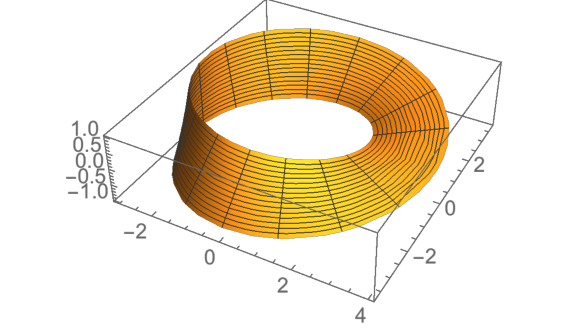
\includegraphics{mobius.pdf}
\end{center}
\end{exercise}

\begin{exercise}{14}
Compute the integrals of the scalar functions below on the parametric surfaces indicated. 
\begin{itemize}
\item[(a)] 
\begin{equation*}
\iint_{S} xy dS, 
\end{equation*}
where $S$ is the surface parametrized by $S(u,v)= 2\cos(u) \textbf{i} + 2\sin(u)\textbf{j} + v\textbf{k}$, for $0 \leq u \leq \frac{\pi}{2}$ and $0 \leq v \leq 1$. 
\item[(b)] 
\begin{equation*}
\iint_{S}  x^2+y^2+z^2 dS, 
\end{equation*}
where $S$ is the surface parametrized by $S(u,v)=u\textbf{i} + v\textbf{j} + (u+v)\textbf{j}$, where $u$ and $v$ are parameters satisfying $u^2+v^2 \leq 1$. 
\item[(c)] 
\begin{equation*}
\iint_S \frac{xy}{z} dS, 
\end{equation*}
where $S$ is the surface parametrized by $S(u,v)=u\textbf{i} + v\textbf{j} + (u^2+v^2)\textbf{k}$, where $u$ and $v$ are parameters satisfying $4 \leq u^2+ v^2 \leq 16$. 
\end{itemize}
\end{exercise}

\begin{exercise}{15}
Decide whether the following properties of the divergence and curl of a vector field (whose components have continuous partial derivatives) are true or false. If they are true, explain why. If they are false, give a counter-example. 
\begin{itemize}
\item[(a)] The curl of a conservative vector field is zero. 
\item[(b)] The divergence of a conservative vector field is zero. 
\item[(c)] The divergence of the curl of a vector field is zero. 
\item[(d)]  The curl of the curl of a vector field is zero. 
\item[(e)] A vector field cannot have both divergence and curl equal to zero.
\end{itemize}
\end{exercise}

\begin{exercise}{16} 
In each of the problems below, use the divergence theorem to evaluate the flux of the vector fields through the closed surfaces below (with respect to outward pointing normal vectors) as triple integrals. 
\begin{itemize}
\item[(a)] The vector field 
\begin{equation*}
F(x,y,z)=x^2z^2\textbf{i}-2y\textbf{j}+3xyz\textbf{k},
\end{equation*}
and the surface of the cube determined by the four vertices $(0,0,0)$, $(0,0,1)$, $(0,1,0)$, $(1,0,0)$. 
\item[(b)] The vector field
\begin{equation*}
F(x,y,z)= xy\textbf{i} + yz\textbf{j} -yz\textbf{k}
\end{equation*}
over the surface composed of the graphs of $z=\sqrt{1-x^2-y^2}$ and $z=0$, on the region where $x^2+y^2 \leq 1$. 
\item[(c)] The vector field 
\begin{equation*}
F(x,y,z)=x(z-y)\textbf{i} + y(x-z)\textbf{j} + z(y-x)\textbf{k} 
\end{equation*}
over the surface of the sphere $x^2+y^2+z^2=16$.
\end{itemize}
\end{exercise}

\begin{exercise}{17}
In each of the problems below, use Stokes' theorem to the evaluate line integrals below as flux integrals over the surfaces indicated. In each case, the curve is oriented counterclockwise when viewed from above. 
\begin{itemize}
\item[(a)]  The line integral
\begin{equation*}
\int_{C} (4xz \textbf{i} + y\textbf{j} + 4xy\textbf{k}) \ dr,
\end{equation*}
over the curve which bounds the surface $S \colon z=9-x^2-y^2, \ z \geq 0$. 
\item[(b)] The line integral 
\begin{equation*}
\int_{C} (x^2\textbf{i} + z^2\textbf{j} -xyz\textbf{k}) \ dr, 
\end{equation*}
over the curve which bounds the surface $S \colon z=\sqrt{4-x^2-y^2}$. 
\item[(c)] The line integral 
\begin{equation*}
\int_{C} [(x-z)\textbf{i} + (y-z)\textbf{j} +x^2\textbf{k}] \ dr
\end{equation*}
over the curve which bounds the portion of the plane $3x+y+2z=12$ on which all three coordinates $x,y,z$ are non-negative. 
\end{itemize}

\end{exercise}

\end{document}
